\chapter{Distributions of Random Variables} \label{ch:rv}

The definition of random variable has been introduced in the previous chapter. This chapter digs deeper into the different types of random variables, their properties, and how the they are described mathematically.

\section{Discrete and Continuous Random Variables}

A random variable may be discrete or continuous depending on the sample space of the variable.

\subsection{Discrete Random Variable}

If a random variable $X$ takes only discrete values $x_1, x_2, ...$, it is called a \mync{discrete random variable}.
The probability of $X$ taking a particular value $x$ is denoted by $P(X=x)$ or simply $f(x)=P(X)$ if no ambiguity. In this case, $P(X=x)$ and $f(x)$ are the probability function (also known as probability mass function) of $X$.

Furthermore, define $P(X\leq x)$ or $F(x)$ as the \mync{cumulative distribution function} of $x$. It is easy to prove that $F(x)$ is nondecreasing, and $\lim_{x\rightarrow -\infty}F(x)=0$, $\lim_{x\rightarrow \infty}F(x)=1$. Also, $F(x)$ ``jumps'' at each $P(X=x_k)>0$ and it is continuous from the right.

\subsection{Continuous Random Variable}

A random variable $X$ may also take continuous values in many applications. For example, let $X$ denote the time consumption to finish a task, in which case $X$ is a random variable whose value can be any positive number.

In this case, the chance for $X$ to take a precise value, say for the student to finish his homework using precisely 25 minutes 13 seconds and 750 milliseconds, is very small (in fact, zero). The probability function $P(X=x)$ becomes pointless. The cumulative distribution function $F(x) = P(X\leq x)$ still makes sense, as it calculates the probability of $X$ given by not a precise value but within a range.

Inspired by this, define \mync{probability density function}[PDF] or $f(x)$ for continuous random variable as follows. 
\begin{eqnarray}
f(x) &=& \dfrac{d}{dx}F(x) \nonumber
\end{eqnarray}
Therefore, $f(x)$ is such that
\begin{eqnarray}
  P(a < X < b) &=& \int_{a}^{b}f(x)dx \nonumber
\end{eqnarray}
and
\begin{eqnarray}
  F(x) &=& P(X\leq x) \nonumber \\
  &=& \int_{-\infty}^{x} f(\epsilon)d\epsilon \nonumber
\end{eqnarray}
Notice that $f(x)$ itself is not probability. It is $f(x)dx$ accumulating in range $x \in (a, b)$ that forms the probability, hence the name ``probability density''.

In science and engineering problems, continuous random variables are more common than discrete random variables. In engineering, discrete random variables can sometimes be described by impulse PDF.

\section{Joint Distribution}

\mync{joint distribution} describes the distribution of multiple random variables combination. It is especially useful when these variables are correlated, in which case the joint probability function or PDF can reflect their correlation. 

For example, in a system identification problem the unknown system parameters are correlated with the measurements and their correlations are described by their joint PDF. System identification tries to estimate the unknown system parameters given the measurements.

\subsection{Joint Probability}

Joint probability considers two or more random variables. For simplicity, consider only two random variables $X$ and $Y$. The same idea can be expanded to more variables.

In the case of discrete variables, define joint probability function and joint cumulative distribution function as follows.
\begin{eqnarray}
  f(x, y) &=& P\left(X=x, Y=y\right) \nonumber \\
  F(x, y) &=& P\left(X\leq x, Y\leq y\right) \nonumber \\
  &=& \sum_{u\leq x}\sum_{v\leq y}f(u, v) \nonumber
\end{eqnarray}

In the case of continuous random variables, let
\begin{eqnarray}
  F(x, y) &=& P(X \leq x, Y \leq y) \nonumber
\end{eqnarray}
be the cumulative distribution function, and joint PDF of $X$ and $Y$ is defined by
\begin{eqnarray}
	f(x, y) &=& \dfrac{d^2}{dxdy}F(x, y) \nonumber
\end{eqnarray}
Therefore,
\begin{eqnarray}
  \int_{x=a}^{b}\int_{y=c}^{d} f(x, y) dxdy &=& P\left(a < X < b, c < y < d \right) \label{eq:jointpdf} \\
  F(x, y) &=& \int_{u=-\infty}^{x}\int_{v=-\infty}^{y}f(u, v)dudv \nonumber
\end{eqnarray}

The cumulative distribution function and PDF of one of the variables, for example $X$, can be derived from the joint PDF as follows. By definition, 
\begin{eqnarray}
	F_X(x) &=& P(X \leq x) \nonumber \\
	&=& \int_{u=-\infty}^{x}\int_{v=-\infty}^{\infty}f(u, v)dudv \nonumber
\end{eqnarray}
Thus,
\begin{eqnarray}
	f_X(x) &=& \dfrac{d}{dx}F_X(x) \nonumber \\
	&=& \int_{y=-\infty}^{\infty} f(x, y) \label{eq:jointpdfdowngrade}
\end{eqnarray}
which is the integration of \eqref{eq:jointpdf} w.r.t. all other variables from $-\infty$ to $\infty$. 

Equation \eqref{eq:jointpdfdowngrade} can be interpreted as follows. If $(X_i, Y_i)$ samples are generated from $f(x, y)$ in \eqref{eq:jointpdf}, and we only look at the $X_i$ of these samples, they should follow \eqref{eq:jointpdfdowngrade}.

\subsection{Conditional Distribution}

Equation \eqref{eq:jointpdfdowngrade} gives the distribution of $X$ regardless of the value of its corresponding $Y$. Conditional distribution, on the other hand, tries to find the distribution of $X$ when $Y$ is measured. For example, in \eqref{eq:jointpdf}, calculate $f_{X|Y}(x |Y=y)$, i.e., the PDF of $X$ given $Y=y$. In many literatures, $f_{X|Y}(x |Y=y)$ is denoted by $f_{X|Y}(x|y)$ for simplicity.

The conditional PDF $f_{X|Y}(x|y)$ can be obtained as follows. It is essentially Bayes' rule applied on continuous variables.
\begin{eqnarray}
  f_{X|Y}(x|y) &=& \dfrac{f(x, y)}{f_Y(y)} \label{eq:conditionalpdf1}
\end{eqnarray}
where $f_Y(y)$ is obtained using \eqref{eq:jointpdfdowngrade}. Equation \eqref{eq:conditionalpdf1} is a function of both $x$ and $y$. Substitute the measured value of $y$ into \eqref{eq:conditionalpdf1} and it reduces to the PDF of $x$ alone. Its integration w.r.t. $x$ from $-\infty$ to $\infty$, therefore, is $1$. This can be easily verified as follows.
\begin{eqnarray}
  \int_{x=-\infty}^{\infty}f_{X|Y}(x|y)dx &=& \int_{x=-\infty}^{\infty}\dfrac{f(x, y)}{f_Y(y)}dx \nonumber \\
  &=& \dfrac{\int_{x=-\infty}^{\infty}f(x, y)dx}{f_Y(y)} \nonumber \\
  &=& \dfrac{f_Y(y)}{f_Y(y)} \nonumber \\
  &=& 1 \nonumber
\end{eqnarray}
Notice that given a particular value of $y$, $f_Y(y)$ is a constant value independent of $x$, hence can be taken out from the integration in the above derivation.

If $X$ and $Y$ are independent variables, $f(x,y) = f_X(x)f_Y(y)$. In this case, \eqref{eq:conditionalpdf1} becomes
\begin{eqnarray}
  f_{X|Y}(x|y) &=& f_X(x) \nonumber
\end{eqnarray}
which implies that the information of $Y=y$ does not affect our understanding of $X$, just as if the information is absent.

Equation \eqref{eq:conditionalpdf1} can be recurrently re-written as
\begin{eqnarray}
f_{X|Y}(x|y) &=& \dfrac{f_{Y|X}(y|x)f_X(x)}{f_Y(y)} \label{eq:conditionalpdf1a}
\end{eqnarray}

\subsection{Parameter Estimation with Conditional Distribution}

Equations \eqref{eq:conditionalpdf1} and \eqref{eq:conditionalpdf1a} are widely used in parameter estimation. Let $\theta$ be the parameter to be estimated, and $x$ the measurement that reflects $\theta$ via measurement model $f(\theta, x)$ which is given in the form of joint PDF. Both $\theta$ and $x$ can be vectors.

Without measurement $x$, the estimate of $\theta$ is given by
\begin{eqnarray}
	\hat{\theta} &=& \int_{-\infty}^{\infty} f_\theta(\theta) d\theta \nonumber
\end{eqnarray}
where $f_\theta(\theta)$ is obtained using \eqref{eq:jointpdfdowngrade}. This is known as the \mync{priori estimation} of $\theta$. 

Given measurement $x$, the \mync{posteriori estimation} of $\theta$ can be obtained as follows. From \eqref{eq:conditionalpdf1a},
\begin{eqnarray}
  f_{\theta|X}(\theta|x) &=& \dfrac{f_{X|\theta}(x|\theta)f_\theta(\theta)}{f_X(x)} \label{eq:conditionalpdf2} \\
  \hat{\theta} &=& \int_{-\infty}^{\infty} f_{\theta|X}(\theta|x) d\theta \label{eq:posterioriestimation}
\end{eqnarray}
where $f_{X|\theta}(x|\theta)$ is known as the \mync{likelihood function} that describes the likelihood of measuring $x$ if the actual parameter(s) is $\theta$. The PDF $f_\theta(\theta)$ is from the priori estimation of $\theta$. Finally, $f_X(x)$ is known as the \mync{evidence}. With fixed $x$, $f_X(x)$ becomes a constant.

Equation \eqref{eq:conditionalpdf2} is essentially
\begin{eqnarray}
  \textup{posteriori} &=& \dfrac{\textup{likelihood}\times\textup{priori}}{\textup{evidence}} \label{eq:posteriorimemo}
\end{eqnarray} 

Terms \textit{priori} and \textit{prior} can be used interchangeably, and so are \textit{posteriori} and \textit{posterior}.

\begin{shortbox}
\Boxhead{Other Parameter Estimation Methods}

Alternative to \eqref{eq:posterioriestimation}, there are at least two other types of commonly seen estimations, namely \mync{Maximum Likelihood Estimation}[MLE] and \mync{Maximum A Posteriori}[MAP].

MLE is given by
\begin{eqnarray}
  \hat{\theta} &=& \argmax_\theta f_{X|\theta}(x|\theta) \nonumber
\end{eqnarray}
whereas MAP is given by
\begin{eqnarray}
  \hat{\theta} &=& \argmax_\theta f_{\theta|X}(\theta|x) \nonumber
\end{eqnarray}

MLE, MAP and \eqref{eq:posterioriestimation} have their advantages and disadvantages, and all of them are widely used in different engineering problems. More about them can be found in Section \ref{sec:mlemap}.

\end{shortbox}

\section{Distribution of Derived Variable}

Let $X$ be a random variable with PDF $f_X(x)$. Let $U$ be another random variable which is a function of $X$, $U=\phi(X)$. The PDF of $U$ can be calculated from $f_X$ and $\phi$. Details are given below.

For simplicity, assume that $U=\phi(X)$ is an injective function (one-to-one function), and $X=\phi^{-1}(U)=\psi(U)$. In that case, the PDF of $U$, $g(u)$, can be obtained as follows.
\begin{eqnarray}
  g(u) &=& \left|\psi\textprime(u)\right|f\left(\psi(u)\right) \nonumber
\end{eqnarray}
For example, let $U=aX$, $X=\frac{U}{a}$.
\begin{eqnarray}
  g(u) &=& \left|\dfrac{1}{a}\right|f\left(\dfrac{u}{a}\right) \nonumber
\end{eqnarray}

Let $X$, $Y$ be two random variables with joint distribution $f(x, y)$. Let $U=X+Y$. The PDF of $U$ can be obtained as follows.
\begin{eqnarray}
  g(u) &=& \int_{-\infty}^{\infty} f(x, u-x)dx \label{eq:conditionalpdf3}
\end{eqnarray}
In the special case where $X$ and $Y$ are independent, $f(x, y) = f_X(x)f_Y(y)$, and \eqref{eq:conditionalpdf3} becomes
\begin{eqnarray}
  g(u) &=& \int_{-\infty}^{\infty} f_X(x)f_Y(u-x)dx \nonumber \\
  &=& f_X * f_Y \nonumber
\end{eqnarray}
where $*$ denotes the convolution operator.

\section{Measure of Distribution}

Given the probability function of a discrete random variable or the PDF of a continuous random variable, a lot of insights can be extracted. Commonly seen measures of a random variable are introduced in this section. Usually, they can be calculated from their associated probability functions or PDFs.

\subsection{Expectation}

In probability and statistics sense, \mync{expectation} (also known as \mync{mean}) describes the average value of a random variable, if the variable is generated many times. For discrete random variable $X$, the expectation is given below.
\begin{eqnarray}
	\textup{E}(X) &=& \sum_{i=1}^{n}x_iP(x_i) \label{eq:expectationdiscrete}
\end{eqnarray}
where $\textup{E}(\cdot)$ is used to denote the expectation, and $n$ the cardinality of the sample space. In the case of countably infinite sample space, replace $n$ with $\infty$ in \eqref{eq:expectationdiscrete}. For continuous random variable, it is
\begin{eqnarray}
	\textup{E}(X) &=& \int_{-\infty}^{\infty}xf(x)dx \label{eq:expectationcontinuous}
\end{eqnarray}
Expectation is sometimes denoted by $\mu$ in literatures.

Some features of expectation calculation are given below.
\begin{eqnarray}
	\textup{E}(cX) &=& c\textup{E}(X) \nonumber \\
	\textup{E}(X+Y) &=& \textup{E}(X) + \textup{E}(Y) \nonumber
\end{eqnarray}
where $c$ is a constant and $X$, $Y$ are two random variables. These features can be easily derived from \eqref{eq:expectationdiscrete} and \eqref{eq:expectationcontinuous}. Furthermore, if $X$, $Y$ are independent, recall $f(x,y) = f_X(x)f_Y(y)$,
\begin{eqnarray}
	\textup{E}(XY) &=& \int_{-\infty}^{\infty}\int_{-\infty}^{\infty} xyf(x, y)dxdy \nonumber \\
	&=& \int_{-\infty}^{\infty}xf_X(x)dx \times \int_{-\infty}^{\infty}yf_Y(y)dy \nonumber \\
	&=& \textup{E}(X)\textup{E}(Y) \nonumber
\end{eqnarray}

\subsection{Variance and Standard Deviation}

\mync{Variance} and \mync{standard deviation} describe how spread samples are from its expectation. It is defined as follows.
\begin{eqnarray}
	\textup{Var}(X) &=& \textup{E}\left(\left(X-\textup{E}(X)\right)^2\right) \label{eq:vardef} \\
	&=& \textup{E}\left(X^2-2X\textup{E}(X)+\textup{E}(X)^2\right) \nonumber \\
	&=& \textup{E}\left(X^2\right)-\textup{E}(X)^2 \label{eq:varderived} \\
	\textup{Std}(X) &=& \sqrt{\textup{Var}(X)} \nonumber
\end{eqnarray}
Variance and standard deviation are sometimes denoted as $\sigma^2$ and $\sigma$ respectively. Notice that \eqref{eq:varderived} also implies that $\textup{E}\left(X^2\right) \geq \textup{E}(X)^2$, a conclusion used in many lemma derivations.

For continuous random variables, from \eqref{eq:varderived} the variance is
\begin{eqnarray}
	\textup{Var}(X) &=& \int_{-\infty}^{\infty} (x-\textup{E}(X))^2f(x)dx \nonumber
\end{eqnarray}

Some features of variance calculation are given below.
\begin{eqnarray}
	\textup{Var}(cX) &=& c^2\textup{Var}(X) \nonumber
\end{eqnarray}
For independent random variables $X$ and $Y$,
\begin{eqnarray}
	\textup{Var}(X\pm Y) &=& \textup{Var}(X) + \textup{Var}(Y) \nonumber
\end{eqnarray}

Mean and standard deviation can be used to standardize a random variable as follows.
\begin{eqnarray}
	X^* &=& \dfrac{X-\mu}{\sigma} \nonumber
\end{eqnarray}
where $\mu$, $\sigma$ are the mean and standard deviation of random variable $X$ respectively. The standardized random variable, $X^*$, has a mean of $0$ and standard deviation of $1$.

\subsection{Moment} \label{sec:moments}

In mathematics, the \mync{$r$-th moment} of a continuous function $f(x)$ about $c$ is defined as follows.
\begin{eqnarray}
	\mu_n &=& \int_{-\infty}^{\infty}(x-c)^nf(x)dx \nonumber
\end{eqnarray}

By simply saying ``moment'' without specifying $c$, it is by default that $c=0$. Let $f(x)$ be a PDF. In this sense, the $0$-th order and the $1$st order moment of a probability density function can be calculated as follows.
\begin{eqnarray}
	&& \mu_0 = \int_{-\infty}^{\infty}f(x)dx = 1 \nonumber \\
	&& \mu_1 = \int_{-\infty}^{\infty}xf(x)dx = \textup{E}(X) \nonumber
\end{eqnarray}
where it can be seen that the $0$th and $1$st moments of a PDF are 1 and its mean, respectively.

Further more, let $c=\mu_1$ be the mean of the random variable to calculate the \mync{$2$nd order central moment} $\mu_2$ as follows.
\begin{eqnarray}
	\mu_2 = \int_{-\infty}^{\infty}(x-\mu_1)^2f(x)dx = \textup{Var}(X) \nonumber
\end{eqnarray}
which is the variance of the random variable.

Using mean and variance to further define \mync{standardized moments} as shown below. Define $\bar{\mu}_k$ for $k\geq 3$ as follows.
\begin{eqnarray}
	&& \bar{\mu}_k = \dfrac{\mu_k}{\sigma^k} \nonumber
\end{eqnarray}
where
\begin{eqnarray}
	&& \mu_k = \textup{E}\left((X-\mu_1)^k\right) = \int_{-\infty}^{\infty}(x-\mu_1)^kf(x)dx \nonumber \\
	&& \sigma^k = \left(\mu_2\right)^{\dfrac{k}{2}} = \left(\int_{-\infty}^{\infty}(x-\mu_1)^2f(x)dx\right)^{\dfrac{k}{2}} \nonumber
\end{eqnarray}
with $\mu_1$ and $\mu_2$ the mean ($1$st order moment) and variance ($2$nd order central moment) of the random variable respectively.

The $3$-rd and $4$-th order standardized moments are known as the \mync{skewness} and \mync{kurtosis} of the PDF respectively. In some literatures, skewness is denoted by $\gamma_1 = \bar{\mu}_3$, and kurtosis $\gamma_2 = \bar{\mu}_4$.

The skewness $\gamma_1$ is a measure of asymmetry of the PDF. When $\gamma_1 > 0$ or positive skew, the distribution has a long tail on the right side of the PDF. When $\gamma_1 <0$ or negative skew, the distribution has a long tail on the left side. When $\gamma_1 = 0$, the PDF might be symmetric (but not necessarily so). Examples are given in Fig. \ref{fig:skewness_demo}.
\begin{figure}[!htb]
	\centering
	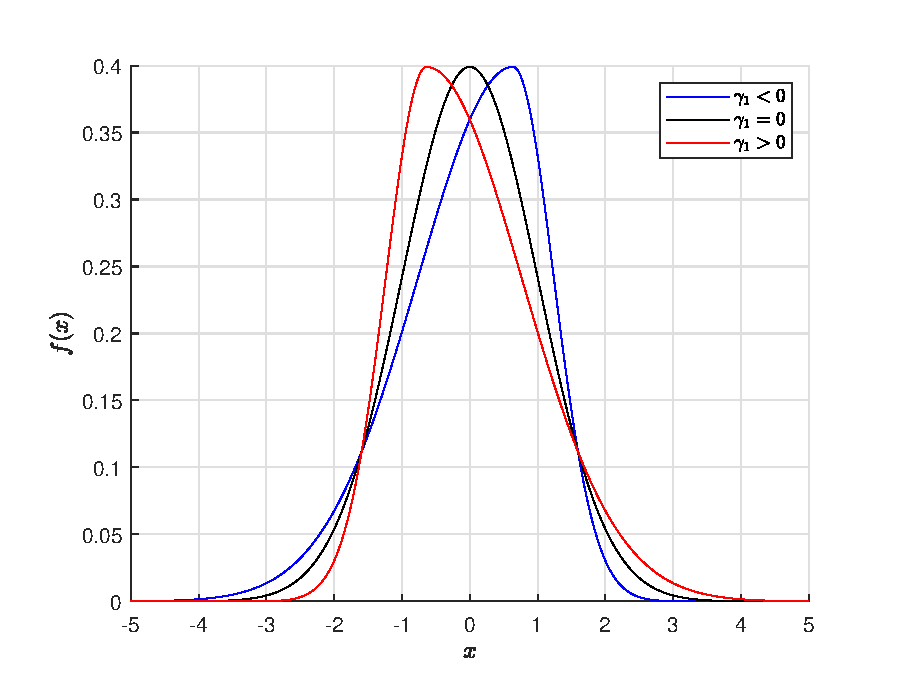
\includegraphics[width=250pt]{chapters/part-1/figures/skewness_demo.eps}
	\caption{Demonstration of PDF with different skewness.} \label{fig:skewness_demo}
\end{figure}

The kurtosis $\gamma_2$ measures the ``tailedness'' of a probability distribution, i.e., whether the PDF has heavy tail or thin tail. The normal distribution, which has $\gamma_2=3$, is often used as a benchmark. Excess kurtosis is kurtosis subtracting $3$, making the normal distribution having the excess kurtosis of $0$. A positive excess kurtosis would mean a ``heavier'' tail than the normal distribution. Examples are given in Fig. \ref{fig:kurtosis_demo}.
\begin{figure}[!htb]
	\centering
	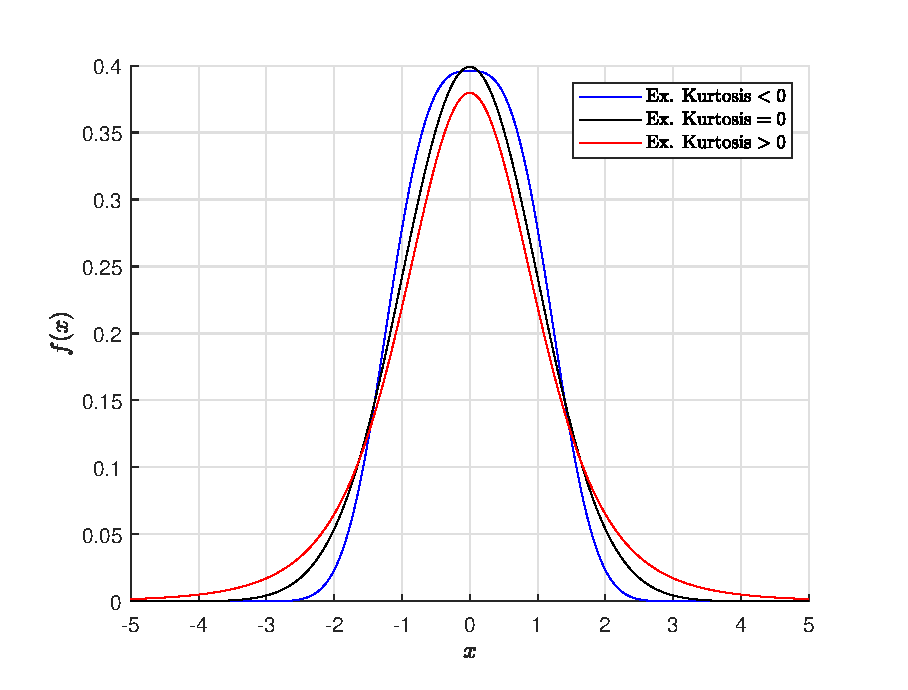
\includegraphics[width=250pt]{chapters/part-1/figures/kurtosis_demo.eps}
	\caption{Demonstration of PDF with different excess kurtosis.} \label{fig:kurtosis_demo}
\end{figure}

\subsection{Covariance and Correlation}

Covariance and correlation are defined for a joint distribution with multiple random variables. For simplicity, consider only two random variables $X$, $Y$ whose joint distribution is given by $f_{XY}(x, y)$. The idea derived from here can be generated to more variables.

The PDF of one variable can be derived from the joint distribution using \eqref{eq:jointpdfdowngrade}. It is straight forward to get the expectation and variance for that variable as follows.
\begin{eqnarray}
	\textup{E}(X) &=& \int_{-\infty}^{\infty}\int_{-\infty}^{\infty}xf(x, y)dxdy \nonumber \\
	\textup{Var}(X) &=& \int_{-\infty}^{\infty}\int_{-\infty}^{\infty}\left(x-\textup{E}(X)\right)^2f(x, y)dxdy \nonumber
\end{eqnarray}

The \mync{covariance} of two variables is defined and calculated as follows.
\begin{eqnarray}
	\textup{Cov}(X, Y) &=& \textup{E}\left((x - \textup{E}(X))(y - \textup{E}(Y))\right) \label{eq:covariance1} \\
	&=& \int_{-\infty}^{\infty}\int_{-\infty}^{\infty}(x - \textup{E}(X))(y - \textup{E}(Y))f(x, y)dxdy \label{eq:covariance2}
\end{eqnarray}
where $\textup{Cov}(X, Y)$ is sometimes denoted by $\sigma_{XY}$. Notice that unlike variance that is always positive, covariance can be zero or negative. If $X$, $Y$ are independent variables, $f(x,y) = f_X(x)f_Y(y)$. From \eqref{eq:covariance2}
\begin{eqnarray}
	\textup{Cov}(X, Y) &=& \int_{-\infty}^{\infty}(x - \textup{E}(X))f_X(x)dx \times \int_{-\infty}^{\infty}(y - \textup{E}(Y))f_Y(y)dy \nonumber \\
	&=& 0 \nonumber
\end{eqnarray}
If the covariance of the two variables is zero, the two variables are called \mync{uncorrelated}. Independent variables are always uncorrelated. However, uncorrelated variables are not necessarily independent.

Furthermore,
\begin{eqnarray}
	\textup{Cov}(X, Y)^2 &\leq& \textup{Var}(X)\textup{Var}(Y) \nonumber
\end{eqnarray}
The proof is given below. Notice that lemma \eqref{eq:explemma} is used in the proof.
\begin{mdframed}[frametitle={Lemma}]
	
	For two random variables $X$ and $Y$,
	\begin{eqnarray}
		\textup{E}(XY)^2 &\leq&  \textup{E}(X^2)\textup{E}(Y^2) \label{eq:explemma}
	\end{eqnarray}
	\noindent Proof:
	\begin{eqnarray}
		0 &\leq& \textup{E}\left(\left(X-Y\dfrac{\textup{E}(XY)}{\textup{E}(Y^2)}\right)^2\right) \nonumber \\
		&=& \textup{E}\left(X^2-2XY\dfrac{\textup{E}(XY)}{\textup{E}(Y^2)}+\textup{E}(Y^2)\dfrac{\textup{E}(XY)^2}{\textup{E}(Y^2)^2}\right) \nonumber \\
		&=& \textup{E}(X^2) - 2\textup{E}(XY)\dfrac{\textup{E}(XY)}{\textup{E}(Y^2)} + \textup{E}(Y^2)\dfrac{\textup{E}(XY)^2}{\textup{E}(Y^2)^2} \nonumber \\
		&=& \textup{E}(X^2) - 2\dfrac{\textup{E}(XY)^2}{\textup{E}(Y^2)} + \dfrac{\textup{E}(XY)^2}{\textup{E}(Y^2)} \nonumber \\
		&=& \textup{E}(X^2) - \dfrac{\textup{E}(XY)^2}{\textup{E}(Y^2)} \nonumber
	\end{eqnarray}
	Therefore
	\begin{eqnarray}
		\dfrac{\textup{E}(XY)^2}{\textup{E}(Y^2)} &\leq& \textup{E}(X^2) \nonumber \\
		\textup{E}(XY)^2 &\leq&  \textup{E}(X^2)\textup{E}(Y^2) \nonumber
	\end{eqnarray}
\end{mdframed}
Using \eqref{eq:explemma} on \eqref{eq:covariance1}, \eqref{eq:vardef} gives
\begin{eqnarray}
	\textup{Cov}(X, Y)^2 &=& \textup{E}\left((x - \textup{E}(X))(y - \textup{E}(Y))\right)^2 \nonumber \\
	&\leq& \textup{E}\left((x - \textup{E}(X))\right)^2\textup{E}\left((y - \textup{E}(Y))\right)^2 \nonumber \\
	&=& \textup{Var}(X)\textup{Var}(Y) \nonumber
\end{eqnarray}
or equivalently
\begin{eqnarray}
	\sigma_{XY}^2 &\leq& \sigma_X^2\sigma_Y^2 \nonumber
\end{eqnarray}
Noticing that while $\sigma_X$, $\sigma_Y$ are always nonnegative, $\sigma_{XY}$ is not,
\begin{eqnarray}
	-\sigma_X\sigma_Y \leq \sigma_{XY} \leq \sigma_X\sigma_Y \label{eq:covlemma}
\end{eqnarray}

The \mync{correlation} of two variables is defined and calculated as follows.
\begin{eqnarray}
	\rho &=& \dfrac{\textup{Cov}(X, Y)}{\sqrt{\textup{Var}(X)}\sqrt{\textup{Var}(Y)}} \nonumber \\
	&=& \dfrac{\sigma_{XY}}{\sigma_X\sigma_Y} \nonumber
\end{eqnarray}
From \eqref{eq:covlemma}, apparently $-1\leq \rho \leq 1$. When two variables are uncorrelated or independent, $\rho=0$. If $\rho=1$, the two variables $X$ and $Y$ are said to be \mync{perfect positive correlated}. This happens usually because the two variables are positively linearly depended, for example, $X=2Y$ or $X=Y+1$. If $\rho=-1$, they are said to be \mync{perfect negative correlated}, and the similar idea applies.

\section{Important Theorems}

There are a few important theorems frequently used in the study of probability and statistics. They are introduced here.

\subsection{Law of Large Numbers} \label{subsec:largenumbers}

The \mync{Law of Large Numbers}[LLN] is a theorem that basically says if performing the same experiment a large number of times, the average of the outcomes of the experiments should eventually converge to a certain value which is the empirical expectation of the experiment. The larger number of trails, the closer the average to the empirical expectation.

In mathematical expression, let $X$ be a random variable which represents the outcome of an experiment. Let $X_i$ be a sample of the outcome. According to LLN,
\begin{eqnarray}
	\lim_{n\rightarrow\infty} \sum_{i=1}^{n}\dfrac{X_i}{n} &=& \bar{X} \nonumber
\end{eqnarray}

\subsection{Central Limit Theorem}

\mync{Central Limit Theorem}[CLT] states the following observation. For \myabb{independent and identically distributed}{i.i.d.} random variables not necessarily following normal distribution, the empirical mean of the samples taken from these distributions tends towards normal distribution when the number of samples is large.

Let $X$ be a random variable not necessarily following normal distribution, and it has mean and variance of $\mu$ and $\sigma^2<\infty$ respectively. Let $X_i$ be samples of the random variable. The empirical mean of the samples is calculated by
\begin{eqnarray}
	\bar{X}_n &=& \dfrac{1}{n}\sum_{i=1}^{n}X_i \nonumber
\end{eqnarray}
CLT states that $\bar{X}_n$ follows normal distribution when $n$ is large. The mean and variance of the normal distribution are $\mu$ and $\dfrac{\sigma^2}{n}$ respectively, i.e.,
\begin{eqnarray}
	\dfrac{\bar{X}_n-\mu}{\dfrac{\sigma}{\sqrt{n}}} \nonumber
\end{eqnarray}
follows standard normal distribution. 

\section{Commonly Seen Distributions}

Commonly seen special distributions are introduced here. Some of them are very useful in statistics analysis and are introduced in more details in later part of the notebook. Both discrete and continuous distributions are considered.

\subsection{Bernoulli and Binomial Distributions}

\mync{Bernoulli distribution} is a discrete probability distribution of random variable $X$ that can take only 2 values, $0$ or $1$. The probability of $X$ taking $1$ is denoted by $p$, while $0$ is $q=1-p$ as shown below.
\begin{eqnarray}
  && f(x) = P(X=x) = \left\{\begin{array}{cc}
                           p & x=1 \\
                           q & x=0
                         \end{array}\right. \nonumber
\end{eqnarray}
subject to $0\leq p \leq 1$, $0\leq q \leq 1$ and $p+q=1$. Each test is also called a \mync{Bernoulli trail}.

The expectation, variance, skewness and excess kurtosis of the distribution are $p$, $pq$, $\dfrac{q-p}{\sqrt{pq}}$ and $\dfrac{1-6pq}{pq}$, respectively.

Run Bernoulli trails repeatedly. Each Bernoulli trail has a probability of $p$ to take value $1$, and $q=1-p$ to take value $0$. The test is carried out $n$ times. The number of the tests with outcome $1$ is a discrete random variable $0\leq X \leq n$. In this case, $X$ follows \mync{binomial distribution}, whose probability function is given by
\begin{eqnarray}
  f(x) &=& P(X=x) \nonumber \\
  &=& \left(\begin{array}{c}
              n \\
              x
            \end{array}\right)p^x(1-p)^{n-x} \nonumber \\
  &=& \dfrac{n!}{x!(n-x)!}p^x(1-p)^{n-x}
\end{eqnarray}

Bernoulli distribution can be taken as a special case of binomial distribution with $n=1$, $x=1$. The expectation, variance, skewness and excess kurtosis of the binomial distribution are $np$, $npq$, $\dfrac{q-p}{\sqrt{npq}}$ and $\dfrac{1-6pq}{npq}$, respectively.

If $n$ is large, Binomial distribution becomes a verification of CLT on Bernoulli trail. Indeed, when $n$ is large, binomial distribution approaches normal distribution.

Binomial distribution can be extended to \mync{multinomial distribution}, where instead of a single event $A$ happening with probability $p$ or not happening with probability $q$, s.t. $p+q=1$, consider multiple events $A_1$, $A_2$, ..., $A_m$, each with probability $p_1$, $p_2$, ..., $p_m$, respectively, s.t. $p_1+p_2+\ldots+p_m=1$. Consider a total of $n$ tests. The number of $A_1$ occurring is a random variable $X_1$, event $A_2$, $X_2$, and so on. Multinomial distribution studies the probability of
\begin{eqnarray}
  P(X_1=x_1, X_2=x_2,\ldots, X_m = x_m) &=& \dfrac{n!}{x_1!x_2!\ldots x_m!}p_1^{x_1}p_2^{x_2}\ldots p_m^{x_m} \nonumber \\
  \textup{s.t.} && \sum x_i = n \nonumber
\end{eqnarray}

Binomial distribution is different from \mync{hypergeometric distribution}. Binomial distribution is used to model ``sampling with replacement'' process: each Bernoulli trail backing up the binomial distribution is i.i.d. and one's result is not affected by its previous trails. Consider picking up a marbles from a bag containing mixture of red and blue marbles whose numbers are given by $r$ and $b$ respectively. Repeat the test $n$ times. After each test, put the marble back to the bag. The number of blue marbles collected is a random variable $X$ that follows binomial distribution
\begin{eqnarray}
f(x) &=& \left(\begin{array}{c}
                        n \\
                        x
                      \end{array}\right)\left(\dfrac{b}{b+r}\right)^x\left(\dfrac{r}{b+r}\right)^{n-x} \nonumber \nonumber
\end{eqnarray}

On the other hand, if after each test the marble is not returned to the bag, it becomes a hypergeometric distribution and the probability follows
\begin{eqnarray}
f(x) = P(X=x) = \dfrac{\left(\begin{array}{c}
                               b \\
                               x
                             \end{array}\right)\left(\begin{array}{c}
                                                       r \\
                                                       n-x
                                                     \end{array}\right)}{\left(\begin{array}{c}
                                                                                 b+r \\
                                                                                 n
                                                                               \end{array}\right)} \nonumber
\end{eqnarray}
with $\textup{max}(0, n-r) \leq x \leq \textup{min}(n, b)$.

When $b$, $r$ are far larger than $n$, the hypergeometric distribution can be approximated by the binomial distribution. When $b$ and $r$ approaches infinity with constant ratio $b/(b+r)$ and $r/(b+r)$, hypergeometric distribution converges to binomial distribution.

\subsection{Normal Distribution}

\mync{Normal distribution}, also known as \mync{Gaussian distribution}, is a continuous distribution. It is one of the most widely used distributions to model random noise. One of the explanations is given as follows. Many measurements such as sensor readings are in fact aggregated values. For example, consider a sensor whose reading refreshes at $1Hz$. Behind the screen, it might be sampling the signal at $1000Hz$, and the reading is the average of every $1000$ samples. According to CLT, the reading shall follow normal distribution.

We will discuss single normal distribution first, followed by joint multivariate normal distribution.

The PDF of the normal distribution is given by
\begin{eqnarray}
  f(x) &=& \dfrac{1}{\sigma\sqrt{2\pi}}e^{-\dfrac{(x-\mu)^2}{2\sigma^2}} \nonumber
\end{eqnarray}
where $\mu$, $\sigma^2$ are the mean and variance of the distribution respectively. The skewness and excess kurtosis of normal distribution are zero.

Let $X$ be a random variable following normal distribution with mean $\mu$ and variance $\sigma^2$. This can be denoted by $X\sim\mathcal{N}(\mu, \sigma^2)$. Let $Z=\dfrac{X-\mu}{\sigma}$, and $Z$ would be a standard normal distribution with mean $0$ and variance $1$.

For a random variable $X$ following normal distribution, the probabilities of its value falling between $\pm \sigma$, $\pm 2\sigma$ and $\pm 3\sigma$ are $0.6827$, $0.9545$ and $0.9973$ respectively. In statistics, sometimes we will take samples with residuals larger than $|3\sigma|$ as outliers.

Multivariate normal distribution describes a vector of random variables $X = \left[X_1, \ldots, X_m\right]$ that follows joint normal distribution. The joint PDF is given by
\begin{eqnarray}
  f(x) &=& \dfrac{1}{\sqrt{(2\pi)^m|\Sigma|}}e^{-\dfrac{(x-\mu)^T\Sigma^{-1}(x-\mu)}{2}} \nonumber
\end{eqnarray}
where $\mu \in \mathbb{R}^m$ is the mean of $x$ and $\Sigma \in \mathbb{R}^{m\times m}$ the covariance matrix. The off diagonal elements in $\Sigma$ describes the correlation of elements in $X$. The $|\Sigma|$ is the determinant of $\Sigma$.

\subsection{Poisson Distribution}

\mync{Poisson distribution} is a discrete probability distribution that takes non-negative integer values $0$, $1$, $2$, $\ldots$. The probability function of poisson distribution is given by
\begin{eqnarray}
  f(x) = P(X=x) = \dfrac{\lambda^xe^{-\lambda}}{x!} \nonumber
\end{eqnarray}
where $\lambda >0$ is the shape parameter as shown in Fig. \ref{fig:poisson_pmf}.
\begin{figure}[!htb]
	\centering
	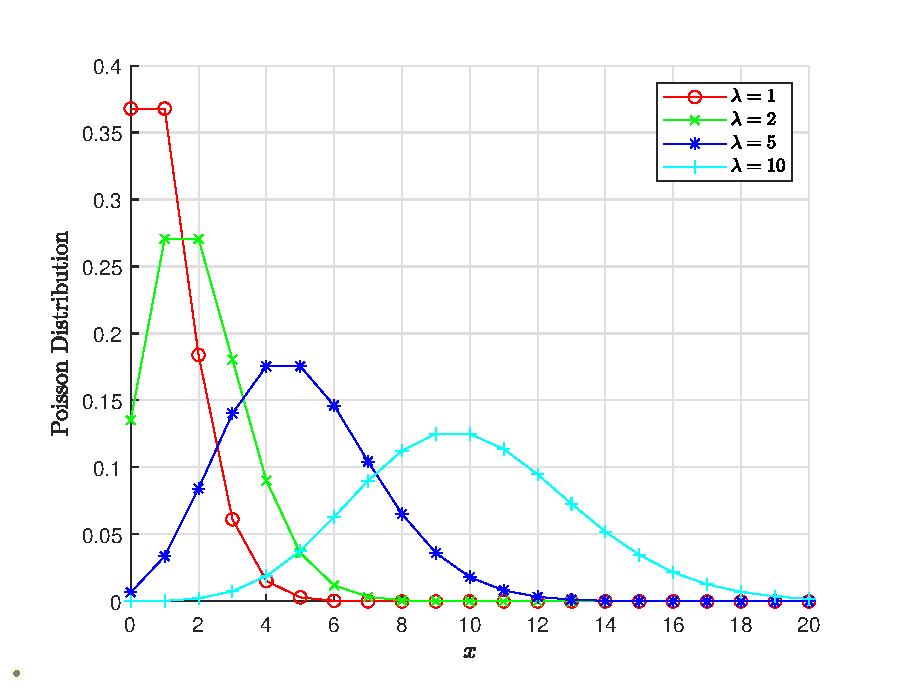
\includegraphics[width=250pt]{chapters/part-1/figures/poisson_pmf.eps}
	\caption{Poisson distribution with different $\lambda$.} \label{fig:poisson_pmf}
\end{figure}
Notice that the sum of two Poisson distribution with shape parameters $\lambda_1$ and $\lambda_2$ is also Poisson distribution with $\lambda = \lambda_1 + \lambda_2$.

Poisson distribution is often used to describe the probability of an event happening a particular number of times in a given window, assuming each occurrence of the event is independent. The parameter $\lambda$ reflects the average number of occurrence. For example, it can model the number of times a machine fails in a year, assuming each failure is independent from another (the failures are completely random and independent). 

Binomial distribution is closely connected with Poisson distribution. Poisson distribution can be taken a limiting case of binomial distribution when $n\rightarrow\infty$, $p\rightarrow 0$ is small, and $\lambda = np$ a decent value. A demonstration is given in Fig. \ref{fig:poisson_vs_b}.
\begin{figure}[!htb]
	\centering
	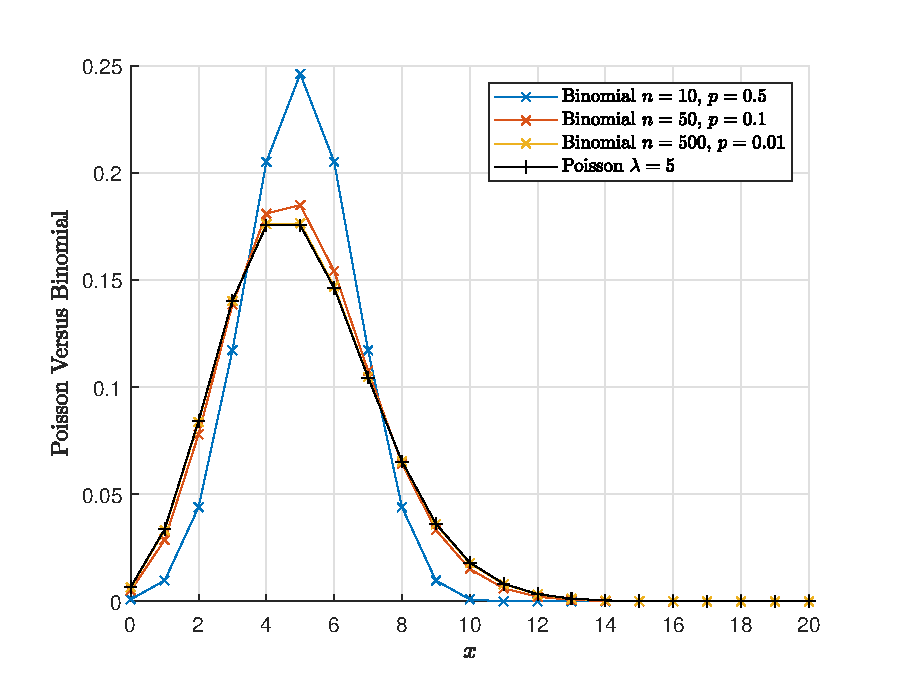
\includegraphics[width=250pt]{chapters/part-1/figures/poisson_vs_b.eps}
	\caption{Poisson distribution approximation using binomial distribution.} \label{fig:poisson_vs_b}
\end{figure}

An intuitive explanation is given using the following example. Consider studying the number of failure of a machine in one year. In each second, the machine has a failure rate of $p$, which of course is very small. The total number of seconds in a year is $31,536,000$, which is a large number and it is associated with the number of trails. The number of failure of the machine in a year can be approximately described by binomial distribution with $n=31536000$. The underlying assumption is that the machine can either fail or survive every second with the probability of $p$ and $1-p$ respectively, and its status in each second are independent, ignoring the downtime of the machine.

Another example of Poisson distribution is the number of visitors of a website in a given period of time. Each internet user has a small probability $p$ to visit the website. The total number of internet users is $n$ which is a large number. The number of visitors to the website follows Poisson distribution with $\lambda=np$ being the expected visitor number.

The expectation, variance, skewness and excess kurtosis of the distribution are $\lambda$, $\lambda$, $\dfrac{1}{\sqrt{\lambda}}$ and $\dfrac{1}{\lambda}$, respectively.

\subsection{Exponential Distribution} \label{sec:exponential_distribution}

\mync{Exponential distribution} can be used to model the duration of time between two events in a Poisson distribution. For example, it can model the operating time of a machine between two failures, assuming that the failures are independent and random.

Exponential distribution is an important special case of the $\Gamma$ distribution. More about $\Gamma$ distribution will be introduced in more details later.

The PDF is the exponential distribution is given by
\begin{eqnarray}
	f(x) &=& \left\{\begin{array}{cc}
		\lambda e^{-\lambda x} & x \geq 0 \\
		0 & \textup{otherwise}
	\end{array}\right. \label{eq:exponential_pdf}
\end{eqnarray}
where $\lambda$ is the shape parameter that reflects the average occurrence rate of the event within a unit time window. Exponential distributions with different choice of $\lambda$ is plotted in Fig. \ref{fig:exponential}.
\begin{figure}[!htb]
	\centering
	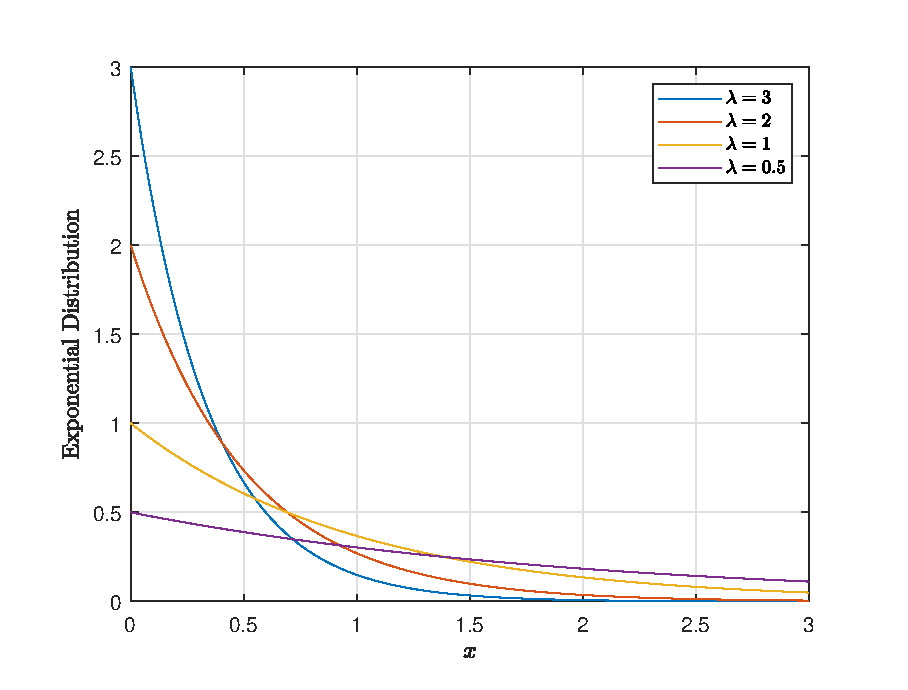
\includegraphics[width=250pt]{chapters/part-1/figures/exponential_pdf.eps}
	\caption{Exponential distributions with different $\lambda$.} \label{fig:exponential}
\end{figure}

The expectation, variance, skewness and excess kurtosis of the distribution are $\dfrac{1}{\lambda}$, $\dfrac{1}{\lambda^2}$, $2$ and $6$, respectively.

\subsection{Uniform Distribution}

Uniform distribution can be either continuous or discrete. Under the scope of this discussion, continuous uniform distribution is studied.

The PDF of continuous uniform distribution is given by
\begin{eqnarray}
  f(x) &=& \left\{\begin{array}{cc}
                    \dfrac{1}{b-a} & a \leq x \leq b \\
                    0 & \textup{otherwise}
                  \end{array}\right. \nonumber
\end{eqnarray}

The expectation, variance, skewness and excess kurtosis of the distribution are $\dfrac{a+b}{2}$, $\dfrac{(b-a)^2}{12}$, $0$ and $-\dfrac{6}{5}$, respectively.

\subsection{Cauchy Distribution}

Cauchy distribution, named after Augustin Cauchy, is a continuous distribution. The PDF is given by
\begin{eqnarray}
  f(x) &=& \dfrac{1}{\pi\gamma\left(1+\left(\dfrac{x-x_0}{\gamma}\right)^2\right)} \nonumber \\ &=& \dfrac{1}{\pi}\dfrac{\gamma}{(x-x_0)^2+\gamma^2} \nonumber
\end{eqnarray}
and it is plotted in Fig. \ref{fig:cauchy_pdf}.

\begin{figure}[!htb]
	\centering
	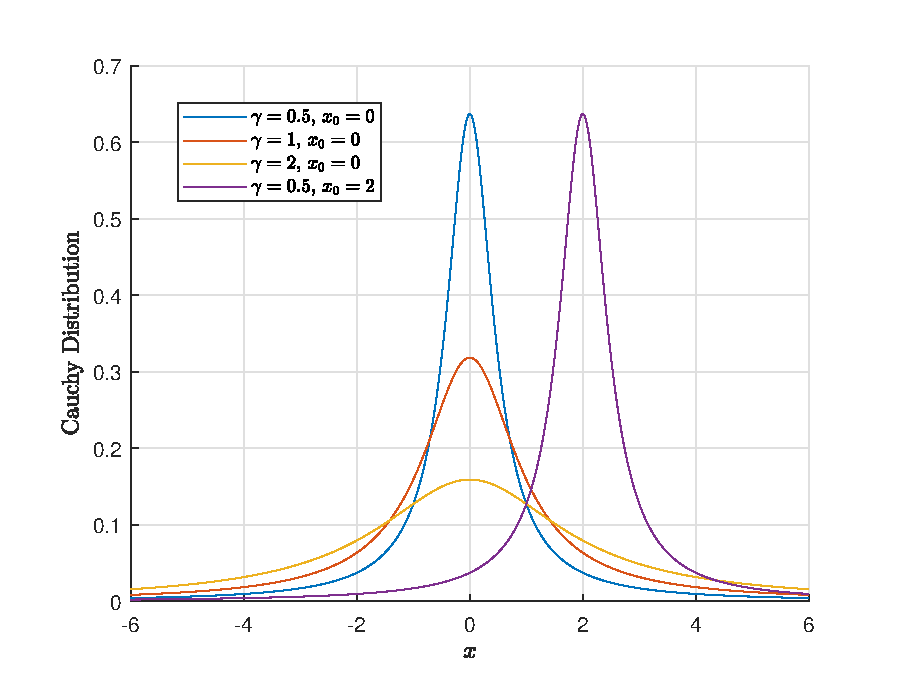
\includegraphics[width=250pt]{chapters/part-1/figures/cauchy_pdf.eps}
	\caption{Cauchy Distribution.} \label{fig:cauchy_pdf}
\end{figure}

From mathematics perspective, Cauchy distribution describes the ratio of two independent normal distributed random variables with mean zero. It is a useful distribution in physics.

\subsection{$\Gamma$, $\chi^2$ and $\beta$ Distributions}

The \mync{$\Gamma$}[gamma], \mync{$\chi^2$}[chi-square] and \mync{$\beta$}[beta] distributions are introduced as follows.

The $\Gamma$ distribution is a continuous distribution with the following PDF
\begin{eqnarray}
  f(x) &=& \left\{\begin{array}{cc}
                    \dfrac{\beta^\alpha}{\Gamma(\alpha)}x^{\alpha-1}e^{-\beta x} & x > 0 \\
                    0 & \textup{otherwise}
                  \end{array}\right. \label{eq:gammapdf}
\end{eqnarray}
where $\alpha>0$ and $\beta>0$ are the shape parameters (some literatures uses scale parameter $\theta = 1/\beta$ in the equation), and $\Gamma(\cdot)$ denotes the Gamma function
\begin{eqnarray}
  \Gamma(\alpha) &=& \int_{0}^{\infty}t^{\alpha-1}e^{-t}dt \nonumber
\end{eqnarray}
for $\alpha > 0$. $\Gamma$ distribution is the superset of many distributions. For example, the exponential distribution introduced in the earlier section is a special case of $\Gamma$ distribution with $\alpha=1$, and it is used to model the time interval between two events in the Poisson distribution.

The plot of the PDF of Gamma distribution is given in Fig. \ref{fig:gamma_pdf}.
\begin{figure}
	\centering
	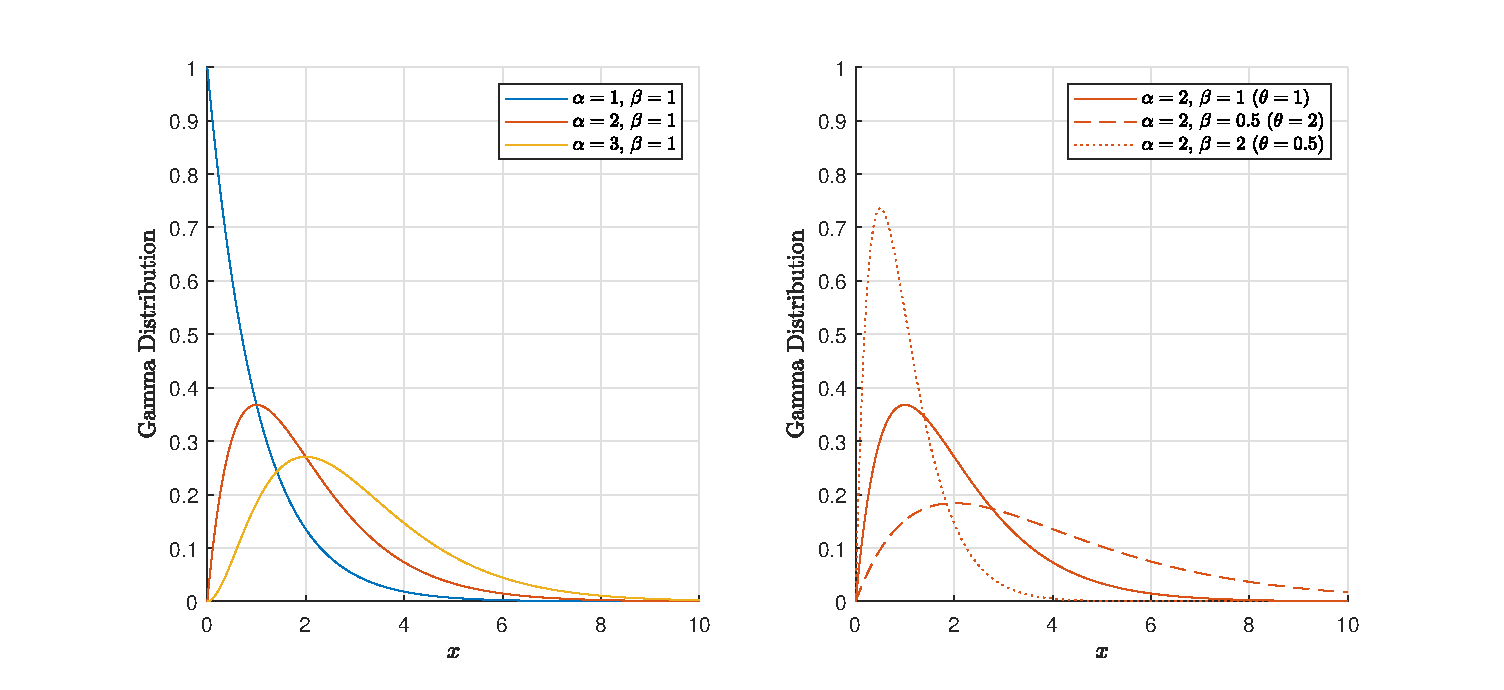
\includegraphics[width=350pt]{chapters/part-1/figures/gamma_pdf.eps}
	\caption{Gamma Distribution.} \label{fig:gamma_pdf}
\end{figure}

\begin{shortbox}
\Boxhead{A Little Bit about Gamma Function}

Gamma function is given by
\begin{eqnarray}
  \Gamma(\alpha) &=& \int_{0}^{\infty}t^{\alpha-1}e^{-t}dt \nonumber
\end{eqnarray}

It is obvious that $\Gamma(1)=1$. If $\alpha > 1$, an integration by parts shows that
\begin{eqnarray}
  \Gamma(\alpha) &=& (\alpha-1)\Gamma(\alpha-1) \nonumber
\end{eqnarray}
Therefore, $\Gamma(\alpha)=(\alpha-1)(\alpha-2)\ldots \times 3 \times 2 \times 1 \times \Gamma(1) = (\alpha-1)!$ for $\alpha \in \mathbb{N}^+$, with $0!=1$.

\end{shortbox}

The expectation, variance, skewness and excess kurtosis of the distribution are $\dfrac{\alpha}{\beta}$, $\dfrac{\alpha}{\beta^2}$, $\dfrac{2}{\sqrt{\alpha}}$ and $\dfrac{6}{\alpha}$, respectively.

The $\chi^2$ estimation is a special case of Gamma distribution. In \eqref{eq:gammapdf}, let $\alpha = \dfrac{r}{2}$ and $\beta=\dfrac{1}{2}$ to get the PDF of $\chi^2$ distribution as follows.
\begin{eqnarray}
  f(x) &=& \left\{\begin{array}{cc}
                    \dfrac{1}{\Gamma(r/2)2^{r/2}}x^{r/2-1}e^{-x/2} & x > 0  \\
                    0 & \textup{otherwise}
                  \end{array}\right. \label{eq:chi2pdf}
\end{eqnarray}
Equation \eqref{eq:chi2pdf} is also denoted by $\chi^2(r)$, where $r$ is known as the degrees of freedom. The plots of PDFs with different $\gamma$ are shown in Fig. \ref{fig:chi2_pdf}.
\begin{figure}
	\centering
	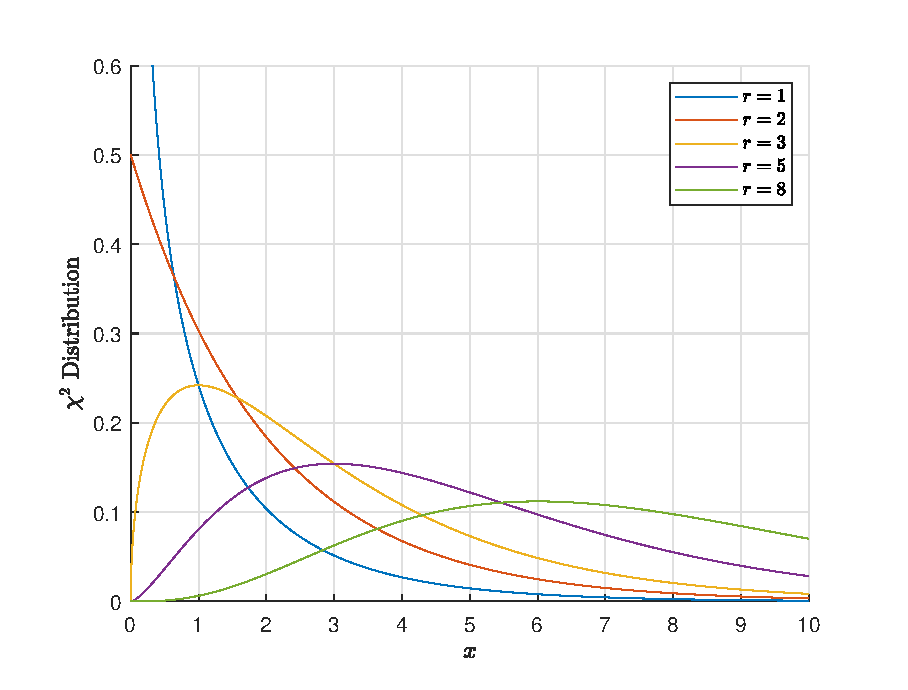
\includegraphics[width=250pt]{chapters/part-1/figures/chi2_pdf.eps}
	\caption{The $\chi^2$ Distribution.} \label{fig:chi2_pdf}
\end{figure}

The $\chi^2$ distribution can be used to model the sum of the squares of $r$ independent standard normal distributions, making it an important distribution is statistics, such as in outlier test. 

The expectation, variance, skewness and excess kurtosis of the distribution are $r$, $2r$, $\sqrt{\dfrac{8}{r}}$ and $\dfrac{12}{r}$, respectively.

Let $X_1$ and $X_2$ be two independent random variables following Gamma distributions with shape parameters $\alpha_1$ and $\alpha_2$ respectively and with $\beta = 1$ in the PDF \eqref{eq:gammapdf}. Denote $X=\dfrac{X_1}{X_1+X_2}$. In this case, $X$ would be a random variable following $\beta$ distribution whose PDF can be derived from \eqref{eq:gammapdf} and it is given by
\begin{eqnarray}
  f(x) &=& \left\{\begin{array}{cc}
                    \dfrac{\Gamma(\alpha_1 + \alpha_2)}{\Gamma(\alpha_1)\Gamma(\alpha_2)}x^{\alpha_1-1}(1-x)^{\alpha_2-1} & 0 < x < 1 \\
                    0 & \textup{otherwise}
                  \end{array}\right. \label{eq:betapdf}
\end{eqnarray}
In some literatures, notation $(a, b)$ or $(\alpha, \beta)$ are used to denote $(\alpha_1, \alpha_2)$ in \eqref{eq:betapdf}.

\subsection{Student's $t$-Distribution}

The zero-mean \mync{Student's $t$-distribution} (also referred as $t$-distribution for simplicity) PDF is given by
\begin{eqnarray}
	f(x) &=& \dfrac{\Gamma\left(\dfrac{\nu+1}{2}\right)}{\sqrt{\nu\pi}\sigma\Gamma\left(\dfrac{\nu}{2}\right)}\left(1+\dfrac{x^2}{\nu\sigma^2}\right)^{-\dfrac{\nu+1}{2}} \label{eq:tpdf}
\end{eqnarray}
where $\nu$ and $\sigma$ are known as the shape and scale parameters respectively. When $\nu\rightarrow\infty$, \eqref{eq:tpdf} reduces to normal distribution. 

The $t$-distribution can also be derived from normal and $\chi^2$ distributions as follows. Let $X_1$ and $X_2$ be two random variables following standard normal distribution and $\chi^2$ distribution with degree of freedom $\nu$. Let
\begin{eqnarray}
	X &=& \dfrac{X_1}{\sqrt{\dfrac{X_2}{\nu}}} \nonumber
\end{eqnarray}
then $X$ follows $t$-distribution \eqref{eq:tpdf}.

Student's $t$-distribution is famous for its heavy-tail characteristics, and it is good at emulating noise with outliers.

The expectation, variance, skewness and excess kurtosis of the $t$-distribution given by \eqref{eq:tpdf} are $0$, $\dfrac{\nu}{\nu-2}$ $(\nu>2)$, $0$ $(\nu>3)$ and $\dfrac{6}{\nu-4}$ $(\nu>4)$ respectively.

\subsection{$F$-Distribution}

Let $X_1$, $X_2$ be two random variables following $\chi^2$ distribution with degree of freedom $\nu_1$ and $\nu_2$ respectively. Let
\begin{eqnarray}
	X &=& \dfrac{\dfrac{X_1}{\nu_1}}{\dfrac{X_2}{\nu_2}} \nonumber
\end{eqnarray}
then $X$ follows $F$-distribution, named after R.A. Fisher.

The PDF of the $F$-distribution is given by
\begin{eqnarray}
	f(x) &=& \left\{\begin{array}{cc}
		\dfrac{\Gamma\left(\dfrac{\nu_1+\nu_2}{2}\right)}{\Gamma\left(\dfrac{\nu_1}{2}\right)\Gamma\left(\dfrac{\nu_2}{2}\right)}\nu_1^{\dfrac{\nu_1}{2}}\nu_2^{\dfrac{\nu_2}{2}}x^{\left(\dfrac{\nu_1}{2}-1\right)}\left(\nu_2+\nu_1 x\right)^{-\dfrac{\nu_1+\nu_2}{2}} & x > 0 \\
		0 & \textup{otherwise}
	\end{array}\right. \nonumber
\end{eqnarray}
where $\nu_1$, $\nu_2$ are the shape parameters of the distribution. 